\documentclass[tikz,border=3pt]{standalone}
\usepackage{fontspec}
\usepackage{amsmath}
\usepackage{xcolor}
\usepackage{tikz}
\usepackage{pgfplots}
\pgfplotsset{compat=1.18}
\usetikzlibrary{arrows.meta,calc,fit,positioning,shapes.geometric,shapes.misc,patterns,plotmarks}
\IfFontExistsTF{Arial}{\setsansfont{Arial}}{\setsansfont{TeX Gyre Heros}}
\renewcommand{\familydefault}{\sfdefault}
\tikzset{
  >={Stealth[length=2.2mm,width=1.5mm]},
  exact title/.style={font=\bfseries\fontsize{10.5}{12}\selectfont,align=center},
  exact subtitle/.style={font=\fontsize{6.3}{7.2}\selectfont,align=center},
  exact label/.style={font=\fontsize{6.4}{7.5}\selectfont,align=center},
  exact tiny/.style={font=\fontsize{5.3}{6.3}\selectfont,align=center},
  panel/.style={draw=black!14,rounded corners=1.2mm,fill=white,line width=.45pt},
  neutral/.style={draw=black!30,fill=black!3,rounded corners=1mm,line width=.45pt},
  arrow/.style={-Stealth,line width=.7pt},
  softarrow/.style={-Stealth,line width=.55pt,draw=black!45},
  dashedarrow/.style={-Stealth,dashed,line width=.55pt,draw=black!55},
  metric/.style={font=\fontsize{5.3}{6.3}\selectfont,fill=white,inner sep=1pt},
}
\newcommand{\pill}[4]{\node[draw=#2!70,fill=#2!10,rounded corners=1.5mm,inner xsep=3pt,inner ysep=2pt,exact label,text=#2] (#1) at #3 {#4};}
\newcommand{\frameboxx}[4]{\draw[draw=#2!65,fill=#2!8,rounded corners=.6mm,line width=.5pt] (#1.south west) rectangle (#1.north east);\node[exact tiny,text=#2] at #3 {#4};}
\newcommand{\axislabel}[3]{\node[exact tiny,text=black!60] at (#1) {#2};\node[exact tiny,text=black!60,rotate=90] at (#3) {#2};}

\definecolor{gblue}{HTML}{4C72B0}\definecolor{gred}{HTML}{E78AC3}\definecolor{gpurple}{HTML}{8D9FCC}\definecolor{ggreen}{HTML}{55A86B}\definecolor{ggray}{HTML}{667085}\definecolor{gink}{HTML}{243447}\definecolor{glight}{HTML}{EEF3F8}\definecolor{gyellow}{HTML}{D6B655}
\begin{document}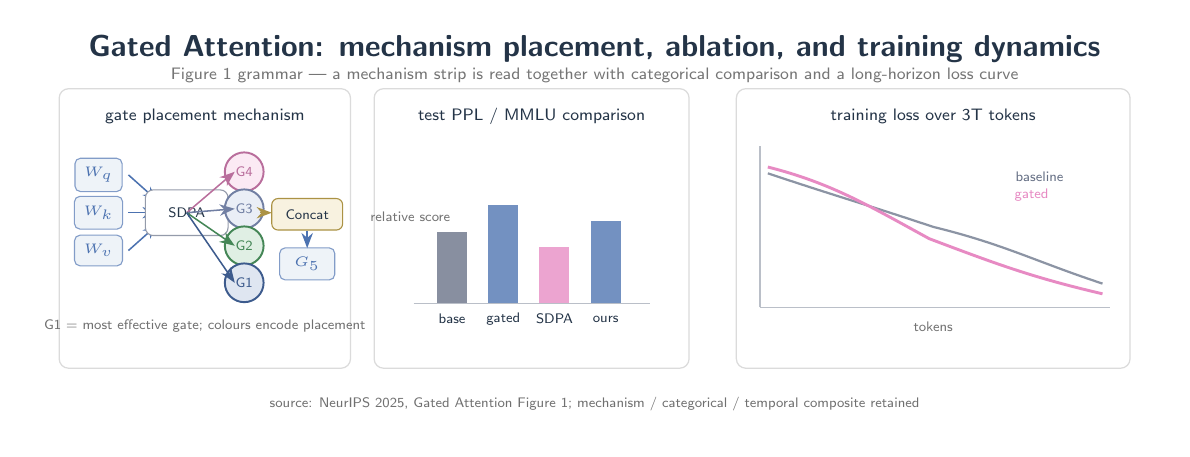
\begin{tikzpicture}[x=1cm,y=1cm]
\path[use as bounding box] (-.2,-2.55) rectangle (14.2,2.55);
\node[exact title,text=gink] at (7,2.28) {Gated Attention: mechanism placement, ablation, and training dynamics};
\node[exact subtitle,text=black!54] at (7,1.94) {Figure 1 grammar — a mechanism strip is read together with categorical comparison and a long-horizon loss curve};
\node[panel,minimum width=3.7cm,minimum height=3.55cm] (mech) at (2.05,0) {};
\node[exact label,text=gink] at (2.05,1.42) {gate placement mechanism};
\node[draw=gblue!70,fill=glight,rounded corners=.7mm,minimum width=.58cm,minimum height=.38cm,exact tiny,text=gblue] at (.7,.68) {\(W_q\)};
\node[draw=gblue!70,fill=glight,rounded corners=.7mm,minimum width=.58cm,minimum height=.38cm,exact tiny,text=gblue] at (.7,.2) {\(W_k\)};
\node[draw=gblue!70,fill=glight,rounded corners=.7mm,minimum width=.58cm,minimum height=.38cm,exact tiny,text=gblue] at (.7,-.28) {\(W_v\)};
\draw[softarrow,draw=gblue] (1.08,.68) -- (1.45,.35);\draw[softarrow,draw=gblue] (1.08,.2) -- (1.45,.2);\draw[softarrow,draw=gblue] (1.08,-.28) -- (1.45,.05);
\node[draw=ggray!70,fill=white,rounded corners=1mm,minimum width=1.05cm,minimum height=.58cm,exact tiny,text=gink] at (1.82,.2) {SDPA};
\foreach \x/\y/\c/\lab in {2.55/.72/gred/G4,2.55/.25/gpurple/G3,2.55/-.22/ggreen/G2,2.55/-.69/gblue/G1}{\fill[\c!18] (\x,\y) circle (7pt);\draw[\c!80!black,line width=.7pt] (\x,\y) circle (7pt);\node[exact tiny,text=\c!80!black] at (\x,\y) {\lab};\draw[softarrow,draw=\c!80!black] (1.82,.2) -- (\x-.12,\y);}
\node[draw=gyellow!80!black,fill=gyellow!18,rounded corners=.8mm,minimum width=.9cm,minimum height=.4cm,exact tiny,text=gink] at (3.35,.18) {Concat};\draw[softarrow,draw=gyellow!80!black] (2.75,.2) -- (2.9,.2);\node[draw=gblue!70,fill=glight,rounded corners=.7mm,minimum width=.7cm,minimum height=.4cm,exact tiny,text=gblue] at (3.35,-.45) {\(G_5\)};\draw[softarrow,draw=gblue] (3.35,-.03) -- (3.35,-.25);
\node[exact tiny,text=black!56] at (2.05,-1.24) {G1 = most effective gate; colours encode placement};
\node[panel,minimum width=4.0cm,minimum height=3.55cm] (bars) at (6.2,0) {};
\node[exact label,text=gink] at (6.2,1.42) {test PPL / MMLU comparison};
\draw[ggray!45] (4.7,-.95) -- (7.7,-.95);\foreach \x/\h/\c/\lab in {5.0/.9/ggray/base,5.65/1.25/gblue/gated,6.3/.72/gred/SDPA,6.95/1.05/gblue/ours}{\fill[\c!78] (\x,-.95) rectangle (\x+.38,-.95+\h);\node[exact tiny,text=gink] at (\x+.19,-1.15) {\lab};}\node[exact tiny,text=black!55] at (4.66,.15) {relative score};
\node[panel,minimum width=5.0cm,minimum height=3.55cm] (curve) at (11.3,0) {};
\node[exact label,text=gink] at (11.3,1.42) {training loss over 3T tokens};
\draw[ggray!45] (9.1,-1) -- (13.55,-1);\draw[ggray!45] (9.1,-1) -- (9.1,1.05);
\draw[ggray!75,line width=.8pt] (9.2,.7) .. controls (10.1,.4) and (10.4,.32) .. (11.3,.02) .. controls (12.2,-.2) and (12.6,-.42) .. (13.45,-.7);
\draw[gred,line width=1.05pt] (9.2,.78) .. controls (10,.58) and (10.5,.28) .. (11.25,-.13) .. controls (12.1,-.45) and (12.55,-.62) .. (13.45,-.83);
\node[exact tiny,text=ggray] at (12.65,.66) {baseline};\node[exact tiny,text=gred] at (12.55,.42) {gated};\node[exact tiny,text=black!55] at (11.3,-1.25) {tokens};
\node[exact tiny,text=black!56] at (7,-2.23) {source: NeurIPS 2025, Gated Attention Figure 1; mechanism / categorical / temporal composite retained};
\end{tikzpicture}\end{document}
